\documentclass[10pt,a4paper]{article}

\usepackage[utf8]{inputenc}
\usepackage[italian]{babel}
\usepackage{amsmath}
\usepackage{amsfonts}
\usepackage{amssymb}
\usepackage{graphicx}

\usepackage[left=2cm,right=2cm,top=2cm,bottom=2cm]{geometry}
\geometry{a4paper}

\usepackage{booktabs} % for much better looking tables
\usepackage{verbatim}
\usepackage{subfig} % make it possible to include more than one captioned figure/table in a single 

\usepackage{fancyhdr} % This should be set AFTER setting up the page geometry
\pagestyle{fancy} % options: empty , plain , fancy
\renewcommand{\headrulewidth}{0pt} % customise the layout...
\lhead{}\chead{}\rhead{}
\lfoot{}\cfoot{\thepage}\rfoot{}

%%% SECTION TITLE APPEARANCE
\usepackage{sectsty}
%\allsectionsfont{\sffamily\mdseries\upshape} % (See the fntguide.pdf for font help)
% (This matches ConTeXt defaults)

% pacchetti che mi fanno schifo e che uso per masochismo
\usepackage[cdot, thickqspace]{SIunits}

\title{Esercitazione 2: Circuito RC - Filtri passivi}
\author{Gruppo BE \\ Alessandro Candido, Roberto Ribatti}
\date{\today} 

\begin{document}
\maketitle

\section{Scopo e strumentazione}
Lo scopo dell'esperienza è:
\begin{itemize}
\item dimensionare opportunamente un filtro passa-basso al fine di migliorare il rapporto segnale rumore nel caso in cui il segnale sia a $\unit{2}{\kilo\hertz}$ e il rumore a $\unit{20}{\kilo\hertz}$ (con un carico a valle di $\sim \unit{100}{\kilo\ohm}$), verificarne quindi la risposta in frequenza;
\item verificare il comportamento in frequenza di un filtro passa banda composto da due filtri RC passa basso e bassa alto in cascata (l'uscita del primo connessa all'entrata del secondo).
\end{itemize}
W
La strumentazione usata è quella presente sul banco di lavoro.
%così suona altamente poco riproducibile, ma dobbiamo trovare una formula per evitare di ripetere ogni volta l'elenco stupido di oscilloscopio, alimentatore, etc.

\section{Filtro passa-basso}

\subsection{Dimensionamento}
Si è dimensionato il circuito tenendo conto dei seguenti criteri:
\begin{itemize}
\item massimizzare il rapporto segnale-rumore;
\item ottenere un segnale abbastanza intenso.
\end{itemize}
Cercare di preservare l'intensità del segnale in ingresso è motivato dal fatto che, se il segnale venisse troppo attenuato dal filtro, gli strumenti per misurarlo introdurrebbero essi stessi un rumore non trascurabile, o comunque sarebbero non trascurabili altri tipi di contributi.

A questo fine si è fissata la frequenza di taglio a $\unit{200}{\hertz}$, infatti minore è la frequenza di taglio maggiore è il rapporto segnale rumore, per cui si otterrebbe un rapporto massimo per una frequenza di taglio nulla. Ma in questo modo si attenuerebbe eccessivamente il segnale, non rispettando il secondo criterio.

\begin{figure}[h!]
	\centering
	\includegraphics[width=0.4\textwidth]{../grafici/SNratio.pdf}
	\caption{Rapporto segnale/rumore}
\end{figure}

A $\unit{200}{\hertz}$ infatti il guadagno è $\sim \unit{-20}{\deci\bel}$ per il segnale, per cui un segnale in ingresso di $\sim \unit{20}{\volt}$ (come quello fornito dal generatore di forme d'onda) viene attenuato a $\sim \unit{2}{\volt}$. In questo modo l'errore introdotto dalla lettura sull'oscilloscopio non è troppo influenzato dal fondo che si osserva in assenza di segnale, la cui intensità stimata è pari a $\sim \unit{2}{\milli\volt}$, quindi lo $0.1\%$ del segnale in uscita.

Per cui si è scelto per il filtro la resistenza $R = \unit{776 \pm 7}{\ohm}$ e il condensatore $C = \unit{1.0 \pm 0.1}{\milli\farad}$. La resistenza è stata scelta anche in modo tale da rendere poco influente la caduta di potenziale sull'impedenza di uscita del generatore. Il valore del carico nella configurazione usata per le misure era $R_{c} = \unit{96 \pm 9}{\kilo\ohm}$

Inoltre si è verificato che il condensatore scelto avesse un'impedenza trascurabile rispetto al carico, in modo da rendere la risposta del circuito indipendente dal valore esatto del carico, ammesso che rimanga dell'ordine di grandezza fissato (o maggiore).

\subsection{Risposta in frequenza}
Dalla teoria sappiamo che il guadagno del filtro passa basso è $|A_v|=1/\sqrt{1+(f/f_0)^2}$ dove $f_0 = 1/(2 \pi RC)$ è detta frequenza di taglio. A questa frequenza il filtro RC ha un guadagno di $\unit{-3}{\deci\bel}$.

Nel nostro caso a partire dal valore misurato di $R$ e dal valore nominale del condensatore $C$, il valore atteso è $f_0 = \unit{200 \pm 20}{\hertz}$ (dove l'incertezza è quasi totalmente determinata dal condensatore).

\paragraph{} Un modo veloce per misurare sperimentalmente questa grandezza è quindi quello di variare la frequenza con continuità fino a trovare  un rapporto $V_{out}/V_{in}$ pari a $1/\sqrt{(2)}$ (ovvero $\unit{-3}{\deci\bel}$). La misura effettuata in questo modo ha prodotto una stima di $f_1 =\unit{208 \pm 10}{\hertz}$.

\paragraph{} Un'altro modo per misurare la frequenza di taglio è eseguire due fit lineari a bassa ed alta frequenza (rispetto a $f_0$ attesa). Calcolando il punto di intersezione e la relativa incertezza (tenendo debitamente conto della covazianza associata alle misure prodotte dai fit) si otterrà la frequenza cercata. I risultati dei fit sono stati: 
\begin{itemize}
	\item prima retta (risposta a bassa frequenza):	 $a=\unit{-0.7 \pm 0.7}{\deci\bel/decade}$,  $b=\unit{2.1 \pm 2.3}{\deci\bel}$ e $c_{ab} = -0.976$, rispettivamente coefficiente angolare, intercetta e coefficiente di correlazione;
	\item seconda retta (risposta ad alta frequenza):	 $c=\unit{-18.2 \pm 0.3}{\deci\bel/decade}$ , $d=\unit{93.6 \pm 2.6}{\deci\bel}$ e $c_{cd} = -0.989$, rispettivamente coefficiente angolare, intercetta e coefficiente di correlazione.
\end{itemize}
L'andamento è quello previsto: la prima retta ha coefficiente angolare e intercetta entrambi compatibili con $0$, come atteso, e la seconda retta ha un'inclinazione di $\sim \unit{-20}{\deci\bel / decade}$.

Il calcolo dell'intersezione produce $f_2 =\unit{ 193 \pm 16}{\hertz}$.
Il grafico dell'intersezione delle rette fittate è riportato di seguito.
\begin{figure}[h!]
	\centering
	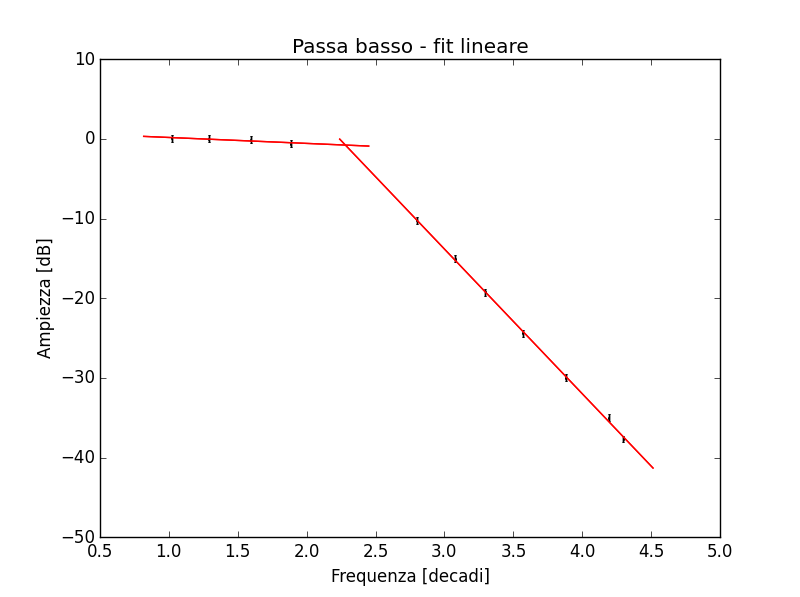
\includegraphics[width=0.6\textwidth]{../grafici/fit_rette.pdf}
	\caption{Grafico dell'intersezione delle rette}
\end{figure}

\paragraph{} La frequenza di taglio può anche essere ottenuta direttamente attraverso il fit della funzione di trasferimento $|A_v|$. Le misure effettuate sono riportate di seguito (insieme a quelle eseguite per il punto precedente).

\begin{figure}[h!]
	\centering
\begin{minipage}[h!]{0.49\textwidth}
	\centering
	\resizebox{\textwidth}{!}{
		\input{../tabelle/tab_Bode_Lowpass_800ohm.txt}}
	\captionof{table}{Dati raccolti del passa basso}
\end{minipage}
\begin{minipage}[h!]{0.49\textwidth}
		\centering
		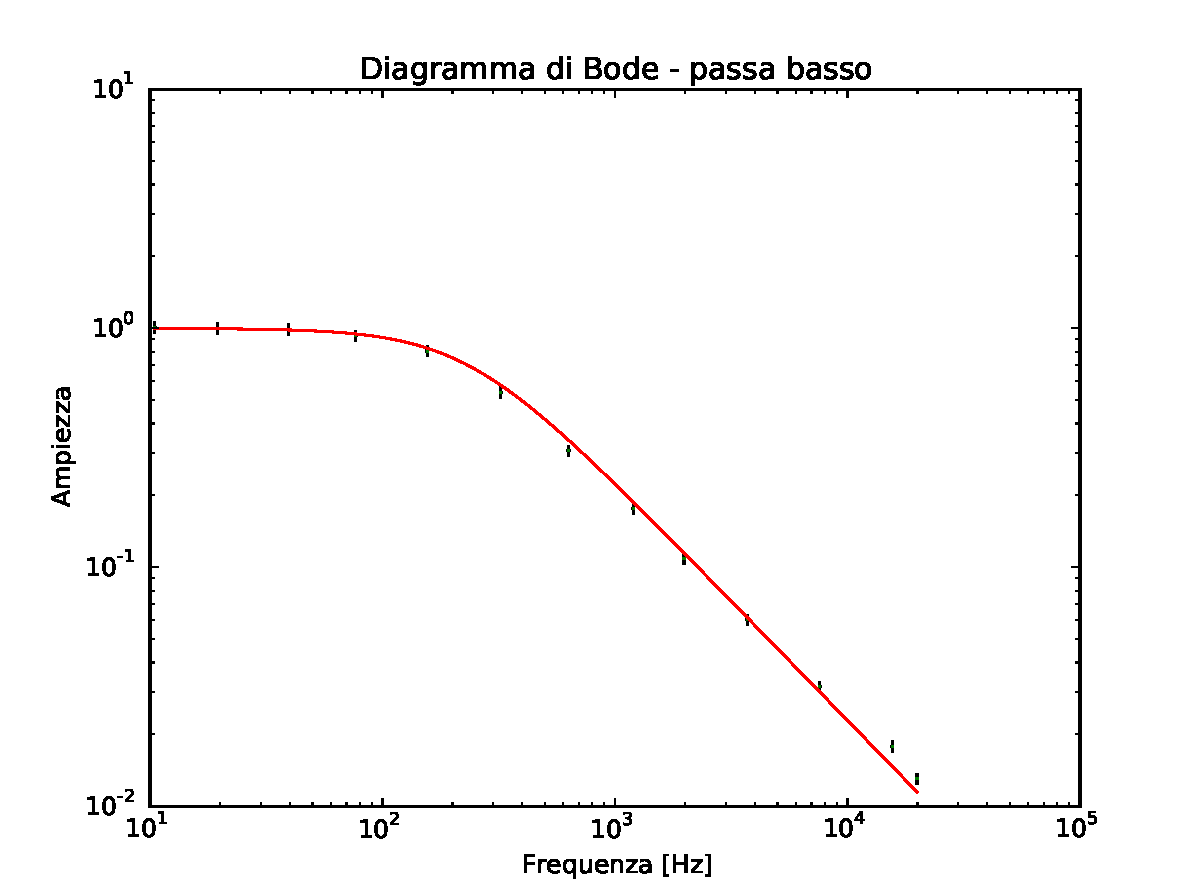
\includegraphics[width=\textwidth]{../grafici/fit_Bode_Lowpass_800ohm.pdf}
		\caption{Misure e fit del passa basso}
\end{minipage}
\end{figure}

La frequenza di taglio fittata è $f_3 = \unit{229 \pm 4}{\hertz}$.

\subsection{Risposta al gradino}
Si è misurato il tempo di carica del condensatore nel circuito in esame, dando in ingresso una funzione a gradino, ottenuta con un'onda quadra di bassa frequenza.\footnote{Se il periodo è abbastanza lungo si può assumere che il condensatore si carichi e si scarichi completamente.}

\begin{figure}[h!]
	\centering
	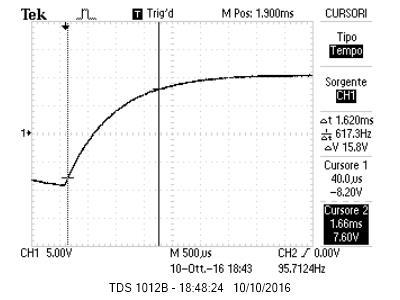
\includegraphics[width=0.5\textwidth]{../oscilloscopio/raise_time.jpg}
	\caption{Tempo di carica del condensatore}
	\label{fig:raise}
\end{figure}

Il valore ottenuto per il tempo di salita del segnale (tra il 10\% e il 90\% del massimo) è $\unit{1.62 \pm 0.06}{\milli\second}$, corrispondente ad una frequenza di $f_4 = \unit{216 \pm 7}{\hertz}$

\subsection{Domande}

\paragraph{Impedenza d'ingresso} L'impedenza d'ingresso è $Z_{in} = R + Z_c(\omega) = R + 1/i\omega C$, quindi:
\begin{itemize}
\item a bassa frequenza l'impedenza diverge;
\item alla frequenza di taglio $Z_{in} = R(1-i)$;
\item ad alta frequenza l'impedenza tende a $R$.
\end{itemize}

\paragraph{Resistenza di carico} L'effetto dell'inserimento di una resistenza di carico è cambiare l'impedenza equivalente del parallelo col condensatore (che in assenza di carico è data dal solo condensatore). In particolare in modulo l'impedenza del parallelo diminuisce, aggiungendo inoltre una parte reale, indipendente dalla frequenza, e quindi modifica i comportamenti asintotici.
Inserendo un carico di $\unit{10}{\kilo\ohm}$ il contributo della resistenza nell'impedenza del parallelo aumenterebbe, e quindi andrebbe tenuto di conto anche a frequenze più basse rispetto al caso con $\unit{100}{\kilo\ohm}$ (ovviamente più basse di circa un fattore $10$).

\subsection{Conclusioni}
Abbiamo quindi ottenuto 5 diverse stime della frequenza di taglio:
\begin{align*}
f_0 &= \unit{200 \pm 20}{\hertz}\\
f_1 &=\unit{208 \pm 10}{\hertz}\\
f_2 &=\unit{ 193 \pm 16}{\hertz}\\
f_3 &= \unit{229 \pm 4}{\hertz}\\
f_4 &= \unit{216 \pm 7}{\hertz}\\
\end{align*}
Sono tutte ragionevolmente compatibili, tranne la misura eseguita con il fit della funzione di trasferimento ($f_3$). 
%Le ragioni di questa discrepanza sono ignote, stronzate a parte !
Si osserva tuttavia negli grafico degli scarti una certa regolarità, questo ci fa pensare che potrebbe esserci una correzione alla funzione di fit, dovuta forse al funzionamento non ideale degli strumenti e del circuito.
Un'altro risultato inatteso, ottenuto dal fit lineare, è la pendenza della retta sulle alte frequenze: $c=\unit{-18.2 \pm 0.3}{\deci\bel/decade}$, che non è in accordo con il risultato teorico $\unit{-20}{\deci\bel/decade}$.

\begin{figure}[h!]
	\centering
	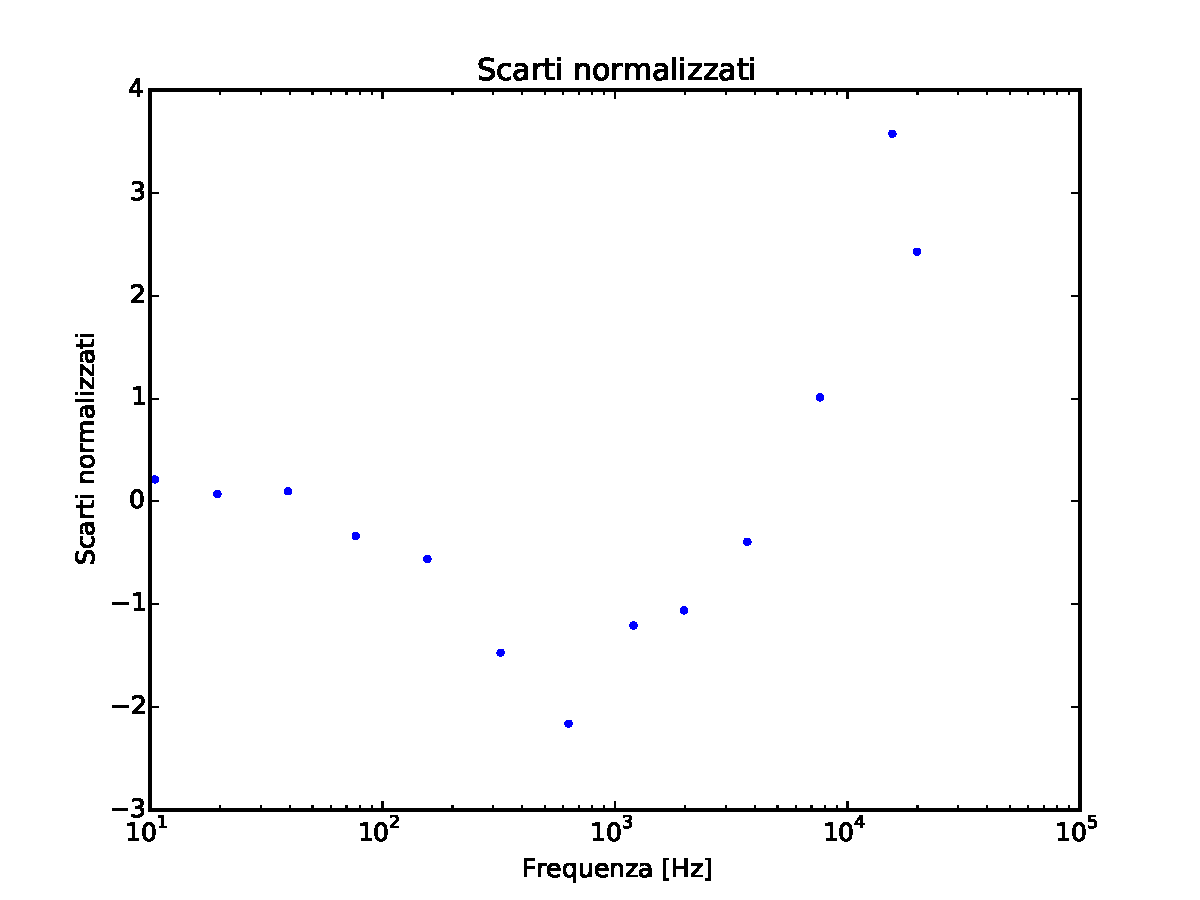
\includegraphics[width=0.5\textwidth]{../grafici/scarti_Bode_Lowpass_800ohm.pdf}
	\caption{Scarti normalizzati fit $|A_v|$ passabasso}
	\label{fig:raise}
\end{figure}

\section{Filtro passa-banda}

\subsection{I stadio: passa-basso}

Si è montato il filtro passa basso come richiesto con una resistenza $R_1 = \unit{3.25 \pm 0.04}{\kilo\ohm}$ (misurata con il multimetro) e un condensatore $C_1=\unit{10 \pm 1}{\nano\farad}$ (valore nominale).

Si è verificato che il filtro seguisse l'andamento generale previsto e che avesse guadagno $\sim 1$ a frequenza $<<f_0$, dove $f_0$ è la frequenza di taglio (in questo caso $l_0 = \unit{4.9 \pm 0.5}{\kilo\hertz}$).

Si è misurata la frequenza di taglio sia cercando la frequenza per cui il guadagno fosse $\unit{-3}{\deci\bel}$ che eseguendo un veloce fit della funzione di trasferimento.
I risultati sono stati:
\begin{itemize}
	\item $l_1 = \unit{4.2 \pm 0.1}{\kilo\hertz}$ con il primo metodo; %propongo di truccare questo dato!
	\item $l_2 = \unit{5.10 \pm 0.14}{\kilo\hertz}$ con il secondo metodo.
\end{itemize}

\subsection{II stadio: passa-alto}
Per il passa alto si è proceduto nella stessa maniera del punto precedente. Si sono usate $R_2=\unit{3.23 \pm 0.04}{\kilo\ohm}$ e $C=\unit{100 \pm 10}{\nano\farad}$, che portano ad una frequenza di taglio $h_0 = \unit{0.49 \pm 0.05}{\kilo\hertz}$.
In questo caso i risultati delle misure sono stati:
\begin{itemize}
	\item $h_1 = \unit{517 \pm 10}{\kilo\hertz}$ con il primo metodo;
	\item $h_2 = \unit{499 \pm 13}{\kilo\hertz}$ con il secondo metodo.
\end{itemize}

I dati raccolti e i grafici dei fit sono qui riportati:

\begin{figure}[h!]
	\centering
	\begin{minipage}[c]{0.49\textwidth}
		\resizebox{\textwidth}{!}{
			\input{../tabelle/tab_Fast_fit_lowpass.txt}}
		\captionof{table}{Dati raccolti passa basso}
	\end{minipage}
\begin{minipage}[c]{0.49\textwidth}
	\resizebox{\textwidth}{!}{
		\input{../tabelle/tab_Fast_fit_highpass.txt}}
	\captionof{table}{Dati raccolti passa alto}
\end{minipage}
\end{figure}

\begin{figure}[h!]
	\centering
	\begin{minipage}[c]{0.5\textwidth}
		\centering
		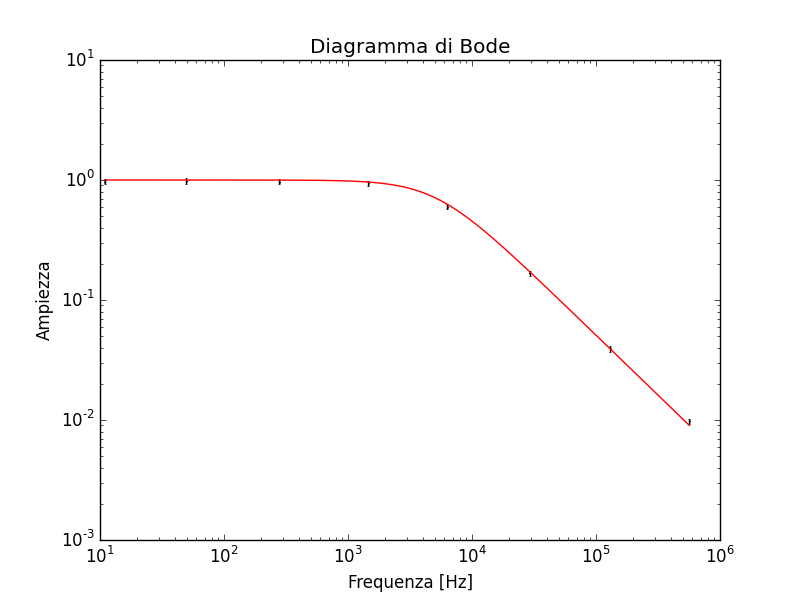
\includegraphics[width=1\textwidth]{../grafici/fit_Fast_fit_lowpass.pdf}
		\caption{Misure e fit passa basso}
	\end{minipage}%
	\begin{minipage}[c]{0.5\textwidth}
		\centering
		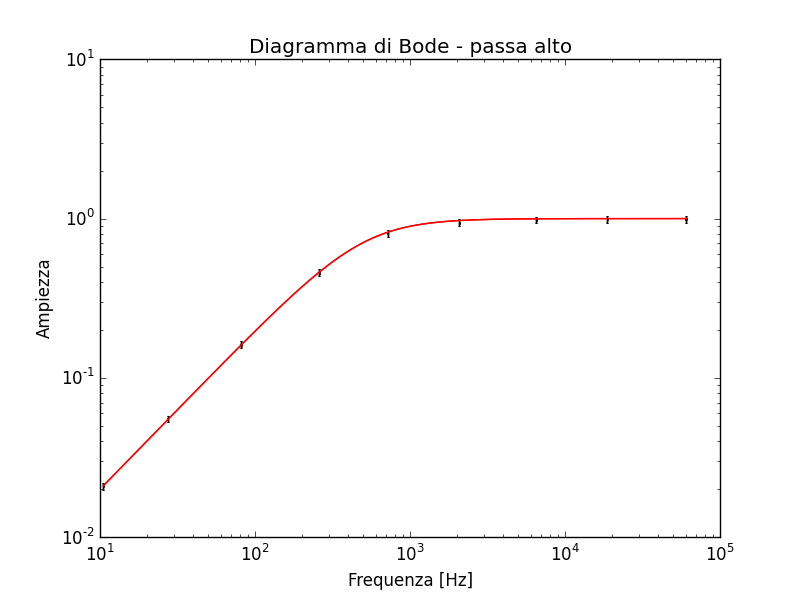
\includegraphics[width=1\textwidth]{../grafici/fit_Fast_fit_highpass.pdf}
		\caption{Misure e fit passa alto}
	\end{minipage}
\end{figure}

\subsection{Configurazione a cascata}
Si è proceduto a mettere in cascata i due filtri prima analizzati per ottenere un filtro passa banda.

Si è analizzato il circuito in 3 bande: bassa frequenza, alta frequenza e centro banda (rispetto alle frequenze $l_0$ e $h_0$) e in queste zone si è proceduto ad un fit lineare. Si sono quindi ottenute le frequenze di taglio attraverso il calcolo delle intersezioni delle rette così ottenute\footnote{L'errore su questa misura è stato ricavato, ovviamente, tenendo conto della correlazione tra i parametri risultato dei fit}.

I risultati dei fit sono stati: (nell'ordine coefficiente angolare, intercetta e coefficiente di correlazione)
\begin{itemize}
	\item prima retta (bassa frequenza): $a=\unit{18.9 \pm 0.5}{\deci\bel/decade}$,  $b=\unit{-52.6 \pm 0.8}{\deci\bel}$ e $c_{ab} =  -0.968$;
	\item seconda retta (centro banda):	$c=\unit{-0.1 \pm 0.6}{\deci\bel/decade}$, $d=\unit{-6.3 \pm 1.9}{\deci\bel}$ e $c_{cd} = -0.996$;
	\item terza retta (alta frequenza):	$e=\unit{-18.54 \pm 0.24}{\deci\bel/decade}$, $f=\unit{66.0 \pm 1.2}{\deci\bel}$ e $c_{ef} =-0.991$.
\end{itemize}
Il guadagno di centro banda è il parametro $d$ fittato.

Le frequenze di taglio misurate attraverso l'intersezione delle rette di fit sono $f_l = \unit{270 \pm 22}{\hertz}$ e $f_h = \unit{8.5 \pm 0.5}{\kilo\hertz}$.
\begin{figure}[h!]
	\centering
	\resizebox{0.6\textwidth}{!}{
	\input{../tabelle/tab_passabanda.txt}}
	\caption{Dati raccolti del filtro passa-banda}
\end{figure}
\begin{figure}[h!]
	\centering
	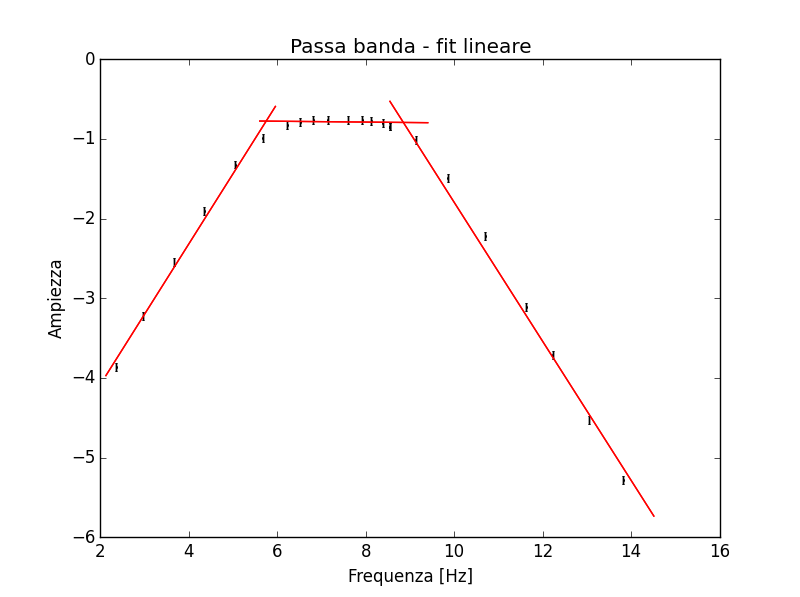
\includegraphics[width=0.7\textwidth]{../grafici/fit_passabandar.pdf}
	\caption{Misure e fit del filtro passa-banda}
	\label{figa9}
\end{figure}

\paragraph{}
Le frequenze ottenute non sono compatibili con quelle misurate sui due filtri presi singolarmente, il motivo è da ricercare nel fatto che il guadagno del passa banda costruito non è il semplice prodotto dei guadagni dei singoli circuiti ma bisogna tener conto delle impedenze di uscita $Z_{out}$ del passa basso e di ingresso $Z_{in}$ del passa alto. Questo particolare potrebbe essere trascurato nel caso in cui $Z_{out} << Z_{in}$, ma non in questo caso in cui sono confrontabili (in particolare uguali).

La teoria ci dice che in questo preciso caso ($R_1 = R_2$) la frequenza di taglio superiore verrà raddoppiata e quella inferiore dimezzata, come in effetti si osserva, e il guadagno massimo (ovvero quello misurato nella banda centrale) si dovrebbe attestare a $\sim \unit{-6}{\deci\bel}$ e anche questo è verificato ($d=\unit{-6.3 \pm 1.9}{\deci\bel}$).

\paragraph{Scelta di $R_1$ e $R_2$} Si poteva scegliere $R_1$ e $R_2$ in modo che il rapporto fra i due fosse approssimativamente nullo, ad esempio scegliendo $R1$ più piccolo oppure $R2$ più grande.
Infatti il guadagno complessivo può essere scritto come il prodotto dei guadagni dei due stadi per un fattore moltiplicativo. Se $A_1, A_2$ sono i guadagni del primo e del secondo stadio, allora:
\begin{equation*}
A_{tot} = A_1 A_2 \frac{1}{1 + \frac{R_1}{R_2} A_1 A_2}
\end{equation*}

\subsection{Conclusioni}
Come scritto nei punti precedenti i risultati delle misure sono in buon accordo con le previsioni.
Fanno eccezione:
\begin{itemize}
	\item la frequenza di taglio del passa basso misurata con i due metodi descritti da due valori non compatibili, probabilmente dovuto a una sottostima dell'errore sul primo metodo, infatti per una piccola variazione (a volte non apprezzabile) del guadagno si hanno in quella zona anche grandi variazioni sulla frequenza;
	\item le pendenze delle rette fittate in \figurename{\ref{figa9}} non sono compatibili con i $\unit{-20}{\deci\bel/decade}$ attesi, come succedeva anche nella sezione precedente. Non è innaturale che il valore risulti minore di quello atteso, infatti la curva ha una pendenza sempre minore del suo asintoto, che corrisponderebbe alla previsione dei $\unit{-20}{\deci\bel/decade}$. Questo problema non era atteso essere però così significativo in quanto i punti scelti per il fit spaziavano fino a diversi ordini di grandezza sopra la frequenza di taglio.
\end{itemize}

\end{document}
